\noindent
\begin{tabular}{cc}
\begin{minipage}{0.65\textwidth}
\begin{exerciseS}[Bilancio di massa: teoria delle reti]
Si consideri  una rete idraulica come quella rappresentata in figura.
All'interno dei tubi scorre acqua. Sia nota le velocit\`a media
dell'acqua all'interno di alcuni dei rami della rete: 
$U_1 = 1\, m/s$, $U_2 = 1.5\, m/s$, $U_3 = 0.5\, m/s$,
$U_7 = 2\, m/s$ e $U_8 = 0.3\, m/s$. 
Il verso della velocit\`a è indicato dalle frecce 
sul disegno.
Determinare la portata volumetrica, la portata in massa e la velocit\`a
media all'interno di ciascun ramo della rete 
sapendo che l'acqua ha una densit\`a pari a $\overline{\rho} = 999\ kg/m^3$,
e che il diametro dei tubi \`e rispettivamente $D_1=0.4\ m$, 
$D_2=0.2\ m$, $D_3=0.2\ m$, $D_4=0.3\ m$, $D_5=0.5\ m$,
$D_6=0.25\ m$, $D_7=0.3\ m$, $D_8=0.6\ m$.

($Q_1 = 0.13\ m^3/s$, $Q_2 = 0.05\ m^3/s$, $Q_3 = 0.02\  m^3/s$, 
 $Q_4 = 0.13\ m^3/s$, $Q_5 = 0.06\ m^3/s$, $Q_6 = 0.13\  m^3/s$, 
 $Q_7 = 0.14\ m^3/s$, $Q_8 = 0.08\ m^3/s$,
 $U_1 = 1\ m^3/s$, $U_2 = 1.5\  m^3/s$, $U_3 = 0.5\  m^3/s$, 
 $U_4 = 1.87\ m^3/s$, $U_5 = 0.29\  m^3/s$, $U_6 = 2.69\  m^3/s$, 
 $U_7 = 2\  m^3/s$, $U_8 = 0.3\ m^3/s$,
 $\overline{Q}_1 = 125.5\  kg/s$, $\overline{Q}_2 = 47.08\  kg/s$,
 $\overline{Q}_3 = 15.69\  kg/s$, 
 $\overline{Q}_4 = 131.8\  kg/s$, $\overline{Q}_5 = 54.49\  kg/s$,
 $\overline{Q}_6 = 131.8\  kg/s$, 
 $\overline{Q}_7 = 141.2\  kg/s$, $\overline{Q}_8 = 84.74\  kg/s$)
\end{exerciseS}
\end{minipage}
&
\begin{minipage}{0.35\textwidth}
   \begin{center}
   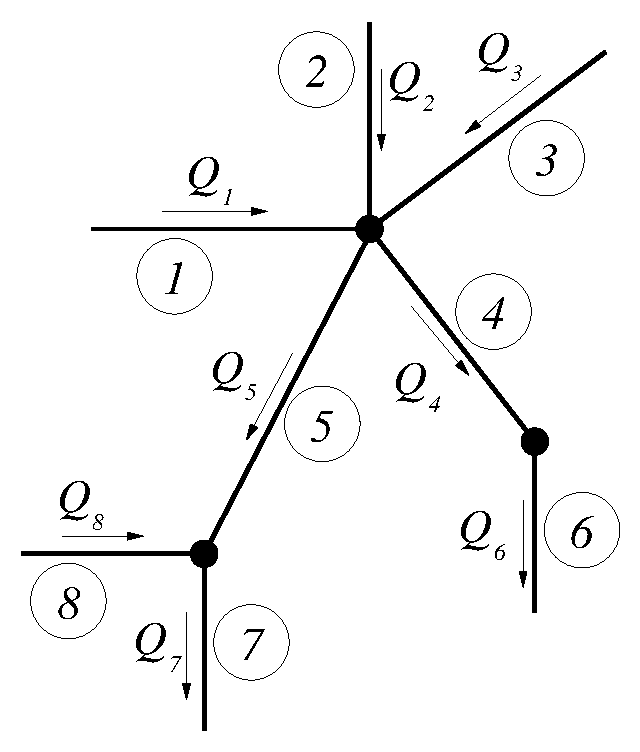
\includegraphics[width=0.90\textwidth]{./fig/rete.eps}
   \end{center}
\end{minipage}
\end{tabular}

\sol

\partone
Bilancio integrale della massa. Teoria delle reti: bilancio ai nodi.

\parttwo
Se il regime di moto è stazionario, la portata massica è costante e indipendente dalla sezione considerata all'interno di ogni singolo tubo. Il bilancio di massa nell'$i$-esimo tubo è,
\begin{equation}
 \underbrace{\dfrac{d}{dt} \int_{V_i} \bm{\rho}}_{=0} = \oint_{S_i} \rho \bm{u} \cdot \bm{\hat{n}} = \oint_{S_{i,{\alpha}}}\rho \bm{u} \cdot \bm{\hat{n}} + \oint_{S_{i,\beta}} \rho \bm{u} \cdot \bm{\hat{n}} = \tilde{Q}_{i,\alpha} + \tilde{Q}_{i,\beta} \quad \rightarrow \quad \tilde{Q}_{i,\alpha} = -  \tilde{Q}_{i,\beta} \ , 
\end{equation}
avendo indicato $S_{i,{\alpha}}$ e $S_{i,{\beta}}$ le due sezioni in ``ingresso'' e ``uscita'' del tubo $V_i$, con $\bm{\hat{n}}$, $\tilde{Q}_{\alpha}$ e $\tilde{Q}_{\beta}$ la normale uscente e i flussi di massa uscenti dal volume $V_i$. Se si calcola il flusso di massa $\overline{Q}_i$ attraverso le sezioni del tubo con normale identificata dal ``verso di percorrenza'' del tubo, uno dei due termini cambia segno e si dimostra che la portata è costante sulle sezioni del singolo tubo, 
\begin{equation}
 \overline{Q}_{i,\alpha} = \overline{Q}_{i,\beta} =: \overline{Q}_{i} \ .
\end{equation}
%
Utilizzando il verso delle frecce indicato in figura per stabilire il segno dei flussi di massa, il bilancio di massa ai nodi porta al sistema lineare,
\begin{equation}
 \begin{cases}
   \overline{Q}_1 + \overline{Q}_2 + \overline{Q}_3 - \overline{Q}_4 - \overline{Q}_5 = 0 & \text{(bil. al nodo in alto)} \\
   \overline{Q}_5 + \overline{Q}_8 - \overline{Q}_7 = 0 & \text{(bil. al nodo a sinistra)} \\
   \overline{Q}_4 - \overline{Q}_6 = 0 & \text{(bil. al nodo a destra)} \ , \\
 \end{cases}
\end{equation}
nel quale le incognite sono i flussi $\overline{Q}_4$, $\overline{Q}_5$, $\overline{Q}_6$, una volta calcolati gli altri flussi con i dati forniti dal testo del problema,
$\overline{Q}_k = \rho \frac{\pi}{4}D_k^2 U_k$, $k=1,2,3,7,8$.
%
Successivamente si calcolano le portate volumetriche $Q_k$ incognite, dividendo le portate massiche $\overline{Q}_k$ per la densità $rho$,
\begin{equation}
 Q_k = \dfrac{\overline{Q}_k}{\rho} \quad , \quad k = 1:8 \ .
\end{equation}

%\begin{equation}
% \begin{cases}
%   Q_1 + Q_2 + Q_3 - Q_4 - Q_5 = 0 & \text{(bil. al nodo in alto)} \\
%   Q_5 + Q_8 - Q_7 = 0 & \text{(bil. al nodo a sinistra)} \\
%   Q_4 - Q_6 = 0 & \text{(bil. al nodo a destra)} \\
% \end{cases}
%\end{equation}

%\item
%Si ricavano le velocità ancora incognite:
%\begin{equation}
%  U_i = \frac{Q_i}{S_i}, \qquad i = 4,5,6
%\end{equation}

%\item
%Infine si calcolano le portate in massa semplicemente moltiplicando 
%quelle volumetriche per la densità $\bar{\rho}$:
%\begin{equation}
%  \bar{Q_i} = \bar{\rho} Q_i, \qquad i = 1:8
%\end{equation}

%\end{itemize}
